%\documentclass{acm_proc_article-sp} 
\documentclass[14pt]{article} 
\usepackage{amssymb,amsmath} 
\usepackage{setspace}
\usepackage{graphicx}
\usepackage{float}
\usepackage{hyperref}
\usepackage{fancyvrb}
\usepackage{color}
\usepackage{algorithm,algorithmic}

%\floatstyle{ruled}
%\newfloat{code}{thp}{lop}
%\floatname{code}{Code}

%\DeclareGraphicsExtensions{.eps}

\definecolor{grey}{rgb}{0.3,0.3,0.3}
\definecolor{prelim}{rgb}{0.1,0.1,0.7}
\newcommand{\preliminary}[1]{\textcolor{prelim}{#1}}
\newcommand{\comment}[1]{}

\graphicspath{{../}}

\begin{document}

\title{DBToaster Server Design Document.}
\author{Anton Morozov, Yanif Ahmad, Christoph Koch.}
\maketitle
\tableofcontents

\newpage
\doublespacing

\section*{Preface}
\subsection*{Formatting conventions.}
This document is a work in progress, text colored \preliminary{as such}
denotes design guidelines that are subject to change, and require input from the
DBToaster developer responsible for the component.

 
\section{Introduction}
DBToaster is a data processing platform supporting continuous query processing of
high-volume update streams through the use of novel compilation techniques to
generate highly specialized and efficient query processing engines.
This document describes the DBToaster Server that provides query processing
functionality, and the administration and management of query and runtime
metadata needed to facilitate processing. The DBToaster Server defines client
interfaces to enable users to specify SQL queries for continuous processing,
specify sources of streaming data for these queries and view query results on
demand. The DBToaster Server executes queries that have been compiled into
native code with the DBToaster Compiler and the LLVM compiler
framework. DBToaster Server internally represents queries as LLVM
\textit{Modules}, which are LLVM bytecode that can be compiled into native code
on demand using just-in-time (JIT) compilation techniques.

\comment{
DBToaster Runtime is a system build based on DBToaster. Runtime provides a stand
alone interface for execution of user defined, DBToaster compiled queries over
specified update streams. Capabilities and usage of the system are demonstrated
on an example of AlgoTrader. AlgoTrader is a platform that simulates Stock
Exchange and serves as a testbed for automatic Trading Algorithms.
}

The DBToaster Server is comprised of three major components: a Compiler Wrapper,
the Data Source Processor and the Query Processor. The DBToaster Compiler
receives SQL queries from a client, compiles them down to executable code and
passes the resulting code to the Query Processor for execution. The Data Source
Processor maintains bookkeeping information for a set of update data streams and
their adaptors (which define stream formats), and hands continuously arriving
tuples to the Query Processor to perform work. The Query Processor runs a set of
queries over given data. The results of each query are made available to
connected clients.

In addition to describing the design of the DBToaster Server, this document presents
an example application built using the DBToaster framework, an algorithmic trading
platform imaginatively named AlgoTrader. 
Algorithmic trading has rapidly become the standard method of trading
equities on electronic exchanges, with the ability to be first-to-market being
critical in determining the success of trading strategies. Thus algorithmic
trading is well-suited to the stream processing model, requiring extremely low
latency computation over update streams. In addition to evaluating algorithmic
trading strategies directly on an orderbook feed from a stock exchange, hedge
funds often wish to test, simulate and analyse trading strategies in a sandbox
prior to live deployment. In short the strategy development cycle may
significantly benefit from having a declarative language to support rapid
prototyping of strategies, and high-throughput and low-latency execution of such
strategies in both simulated and deployed environments.

The AlgoTrader platform is intended to represent a suite of tools for a
quantitative analyst to develop his/her trading strategies, including strategy
programming tools, strategy execution and administration, and simulation and
testing tools where strategies can be evaluated against a simulation of an
electronic stock exchange.
The AlgoTrader platform consists of two components: a Stock Exchange Simulator
and Trading Algorithm Engine. The Stock Exchange Simulator implements a
realistic simulation of an Electronic Communication Network (ECN). Each ECN
serves as a matchmaker between stock buyers and sellers. The Trading Algorithm
Engine is a testbed for developing automatic trading strategies. Each strategy
runs a set of queries over data streams coming from Stock Exchange
Simulator. Based on query results, trading strategies either buy or sell stocks.

We present an overall architecture diagram showing both the DBToaster Server and
AlgoTrader platform in Figure \ref{fig:overview}.

\comment{
Data Sources components are a source of the incoming data. The end user
applications need these data to be processed by running various queries over
it. In this particular example we will be using an Exchange Simulation Server
application as a data source. Next component is the Algorithms Simulation
Engine. This component is the end user program of interest. It is responsible
for the decision making and outside influences (i.e. what ever user needs to be
done with the help of the queries over the data streams). In out example it is a
Trading Runtime Platform. The last component is DBToaster Runtime. The component
is responsible for collecting the data from various data sources specified by
the users, running appropriate queries over the data and conveying the query
results to Algorithms Simulation Engine.
}

\comment{
The the flow of information between the three components is as follows. Once
started data generation component generates data, these data comes from a
variety of sources stock exchange, sensor network, remote applications etc. The
data comes as a continuous stream of information, this information is presented
in a well known format. In many of the cases it is possible that the end user
does not have much control over the data stream but the ability to listen to the
incoming data. These data is sent to DBToaster runtime. The runtime is
responsible for collecting data from those data sources and running a dynamic
set of user defined queries over these data. The queries are dynamically loaded,
compiled and if needed removed during the execution of a runtime. The results of
the queries are forwarded to Algorithms Simulation Engine (a.k.a the end
user). The Engine's job is to get the data from the runtime. Based on the
results of the queries Algorithm Engine performs tasks needed by the users. In
our example, based on the information received Algorithm Engine buys and sell
stocks on a NASDAQ exchange simulator.
}

\comment{
The particular application we have chosen to demonstrate the capabilities and
performance of our system is a NASDAQ trading simulation. In this simulation
there is a set of servers; each server arranges stock exchanges between
different trading parties. The results of those exchanges as well as information
about interest in stock sells and purchases is transmitted to all parties
interested in such information. Based on these information different trading
algorithms decide to buy and sell stocks. The arrangement of all the components
in the Trading system can be seen in figure \ref{fig:overview}.
}

\begin{figure}
  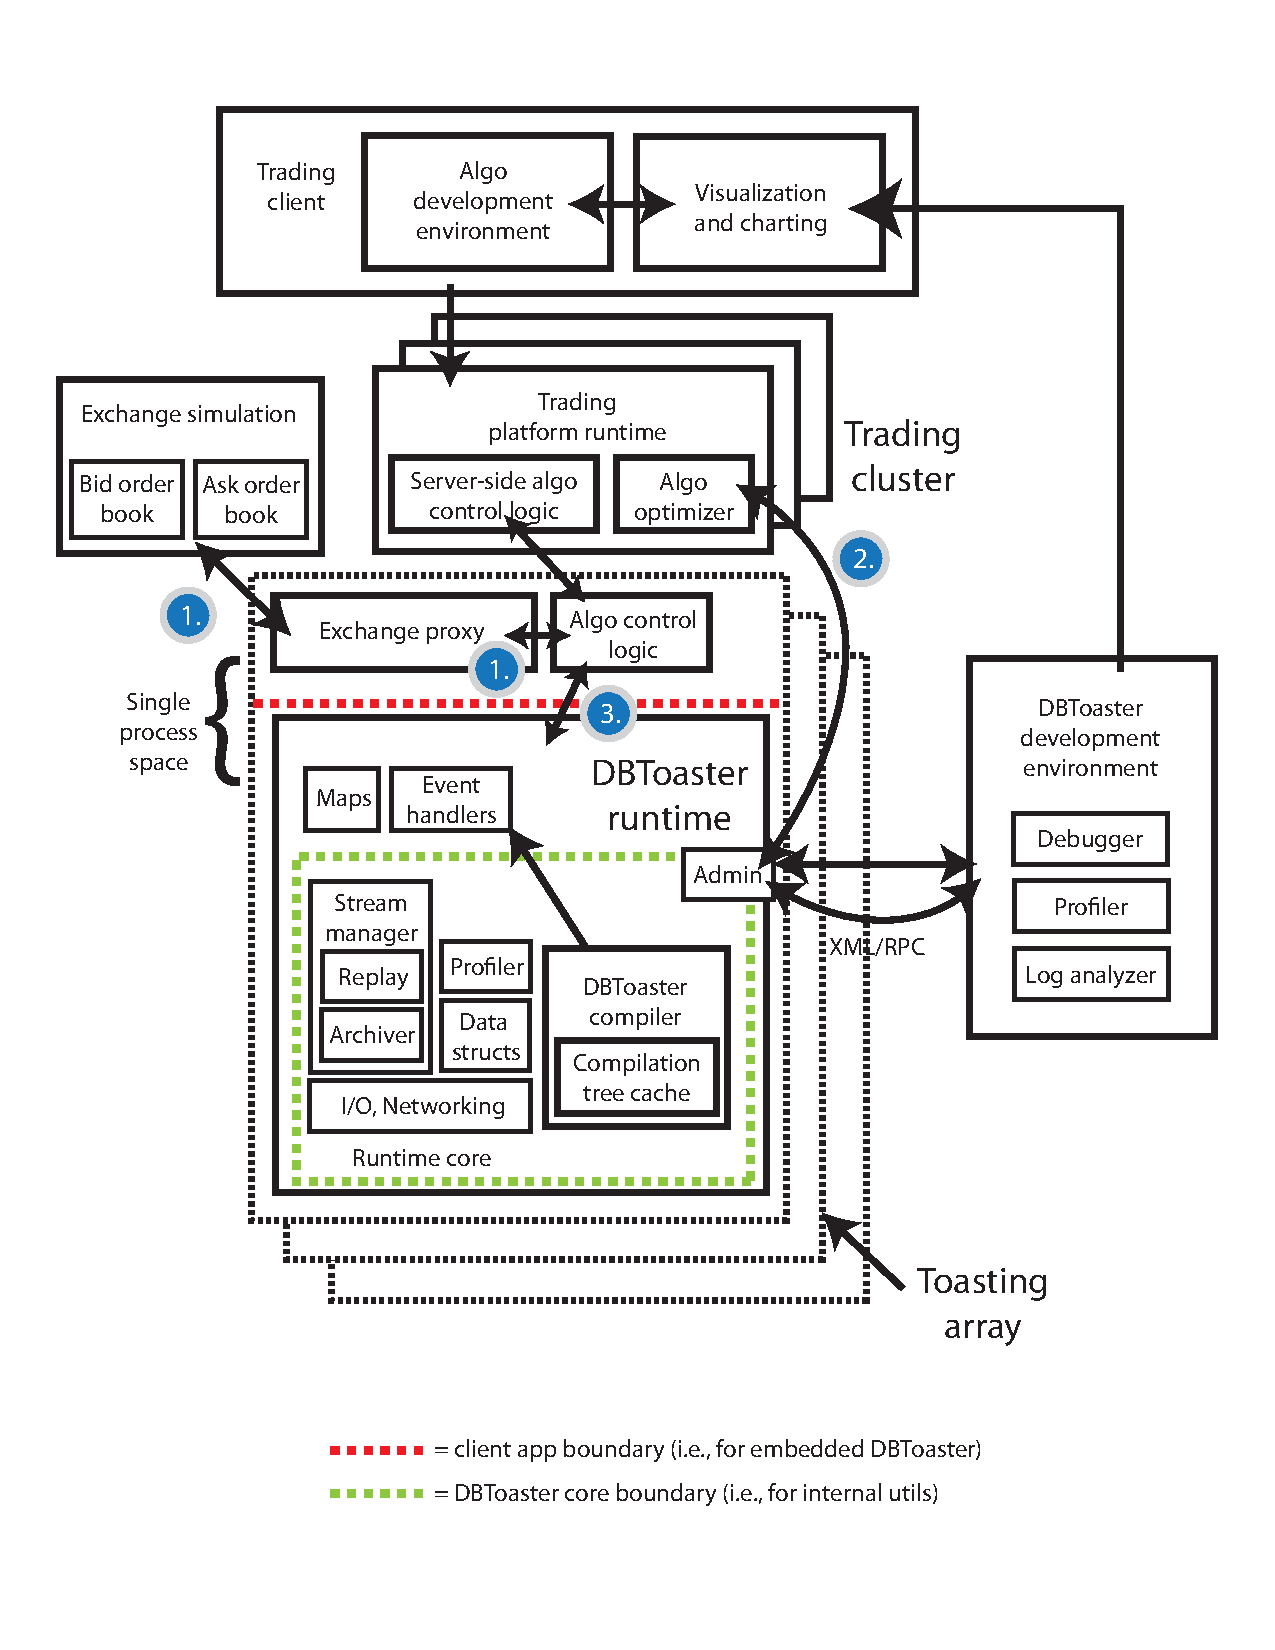
\includegraphics[width=4.50in]{figures/finapp.pdf}
  \caption{Runtime and AlgoTrader Interactions.}
  \label{fig:overview}
\end{figure}

%description of particularities of the system


\section{DBToaster Server}

The DBToaster Server manages the creation, administration and execution of
queries. In this section we describe the core components of the server,
including their responsibilities. These core components include the Compiler
Wrapper, Query Processor and Data Source Processor. The Compiler is responsible
for \textit{toasting} SQL queries, that is generating native code from SQL
queries submitted to the system. The Compiler is also responsible for generating
data source and adaptor code. Adaptors are responsible for loading and feeding
data into a query, and enables highly efficient formatting and parsing of data
from a file source or a network source. We describe data sources and their
adaptors in more detail later.

The Query Processor is the heart of the DBToaster Server and handles the
scheduling and execution of queries represented as native code. The DBToaster
Server Query Processor is designed under a multi-threaded paradigm, enabling
concurrent execution of queries with the aid of a thread pool.  We discuss the
limitations of our concurrency model, as well as the locking model for handing
data to queries for processing, and maintaining a schedule of runnable queries.

The Data Source Processor is responsible for administering input data for the
DBToaster Server, by managing file and network sources, and the adaptor code
associated with each source. The Data Sources Processor uses a multithreaded
model, via a thread pool, to format input data into a structured type for
DBToaster queries. Thus the Data Source Processor performs the low-level reading
and writing of bytes from a file or network data source, executes adaptor code
on the bytes read, and hands the new input to the DBToaster Server Query
Processor. By supporting query-specific adaptors, we provide flexibility in the
data formats that may be used for query processing, both including standard
adaptors such as CSV, XML file or network source adaptors, as well as enabling
query developers to write their own adaptors.

A pictorial representation of DBToaster Runtime can be found in Figure~\ref{fig:dbt-runtime}.

\comment{
DBToaster Server consists of three major components: Compiler, Query Processor
and Data Sources Processor. Each of these components also interacts with each
other. The complete representation of DBToaster Runtime can be found in figure
\ref{fig:dbt-runtime}.

Each of three components interacts with external environment. Compiler and Query
Processor both implement a server to interact with users. Compiler receives SQL
queries and data adaptors. Query Processor uses server to distribute query
results to users. Data Sources Processor creates user specified clients to
receive data from a variety of sources.
}

\comment{
Compiler receives requests from the client to instantiate a Data Source Reader
for receiving data or a SQL query to process data. The created Data Reader is
passed to the Data Source Processor and a Query is passed to Query Processor to
run on the data.
}

\begin{figure}
  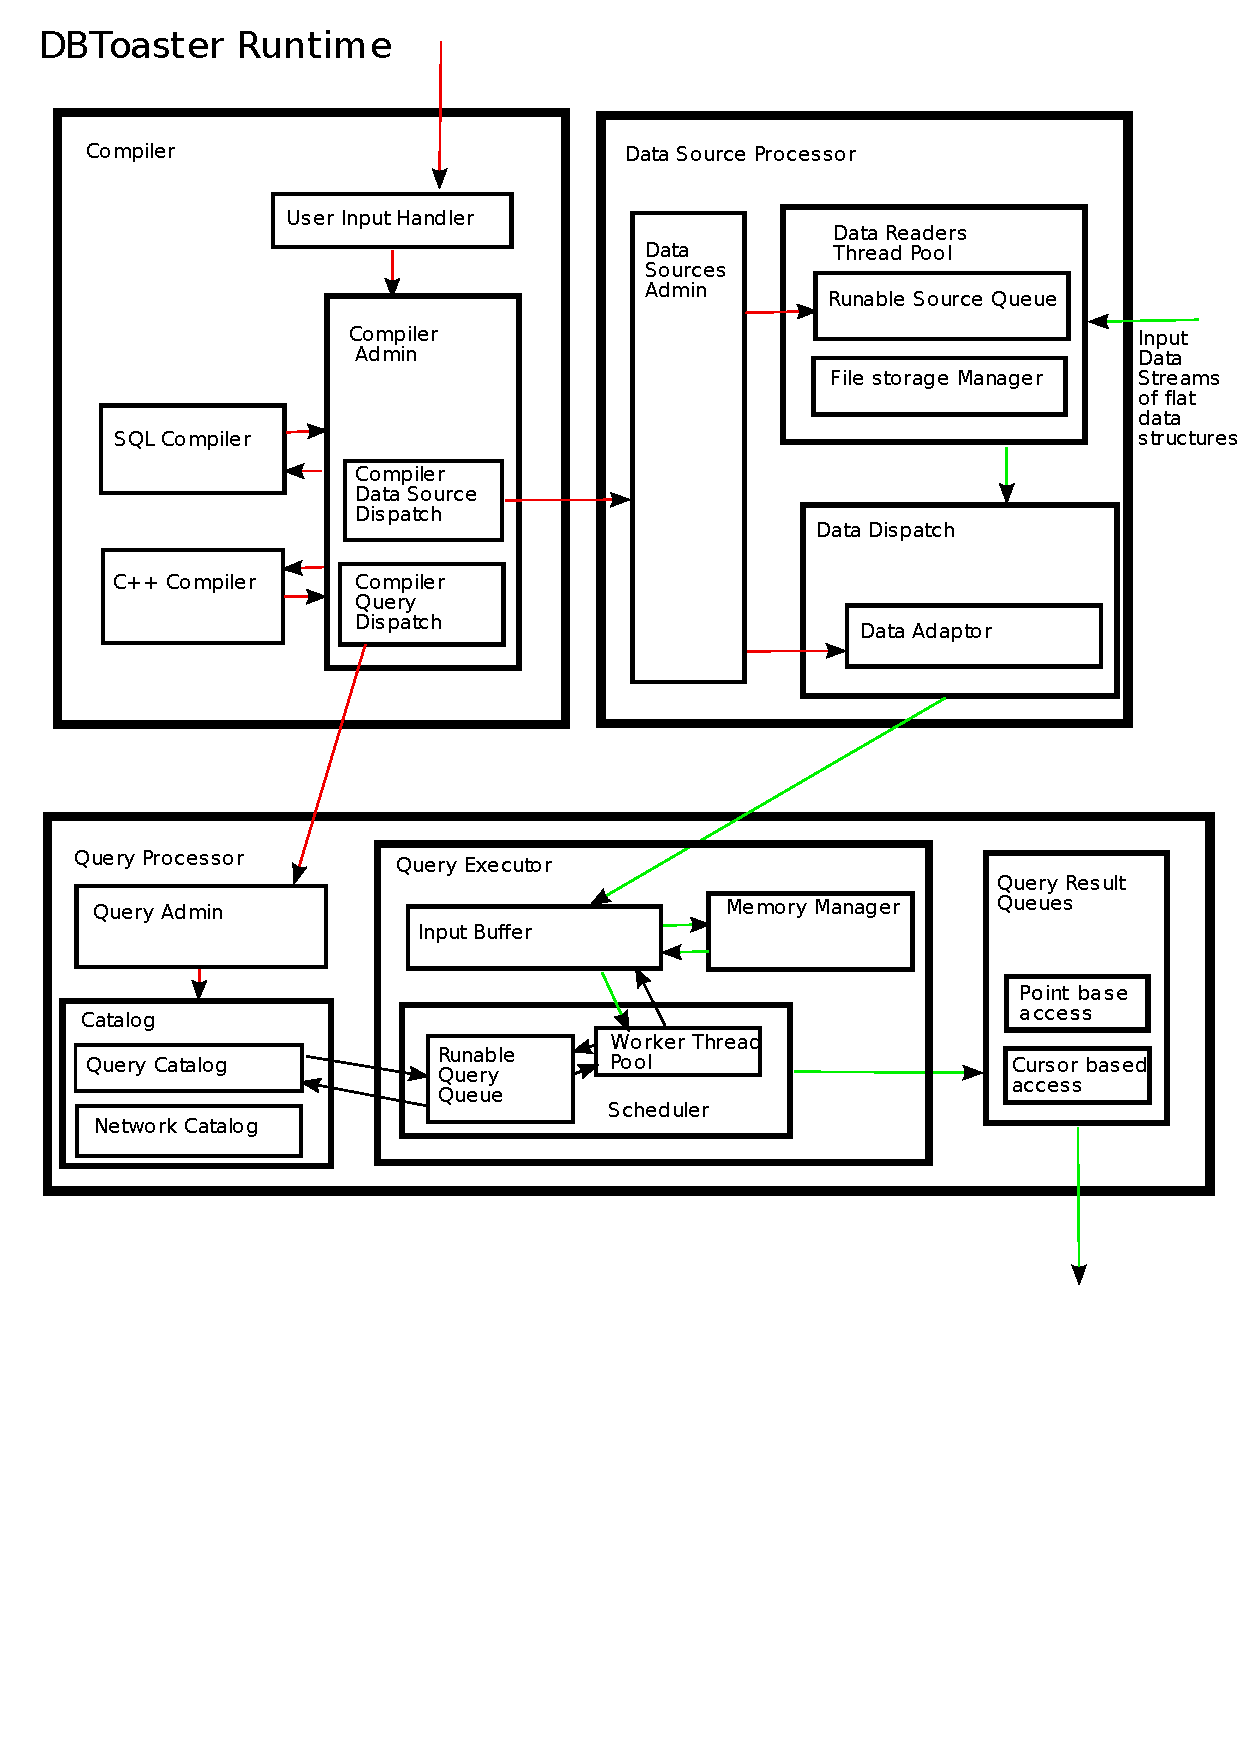
\includegraphics[width=4.50in]{figures/DBToasterRuntime.pdf}
  \caption{DBToaster Structure.}
  \label{fig:dbt-runtime}
\end{figure}



\subsection{DBToaster Compiler Wrapper}

The DBToaster Compiler Wrapper generates native code from SQL queries, where by
native code we refer to LLVM Modules. We refer the reader to the LLVM
documentation \cite{url-llvm} for more detail on these Modules. The Compiler
Wrapper component in the DBToaster Server is a wrapper which invokes the
DBToaster compiler on a SQL statement, or a SQL file.  The wrapper compiler's
subcomponents are shown in Figure~\ref{fig:wrapper-compiler}.  The Compiler
Admin provides the interface for DBToaster clients to submit queries for
execution to the system. It also manages the compilation and deployment of
queries into the Data Source Processor and Query Processor.  The SQL compiler is
written in OCaml and generates C++ source code consisting of \textit{event
handler} functions. We briefly describe the structure of the C++ source code
below. The C++ source is then compiled to native code using an LLVM
compiler. For the time being this is \texttt{llvm-g++}, due to \texttt{clang}'s
\cite{url-clang} limited support for C++.

\begin{figure}
  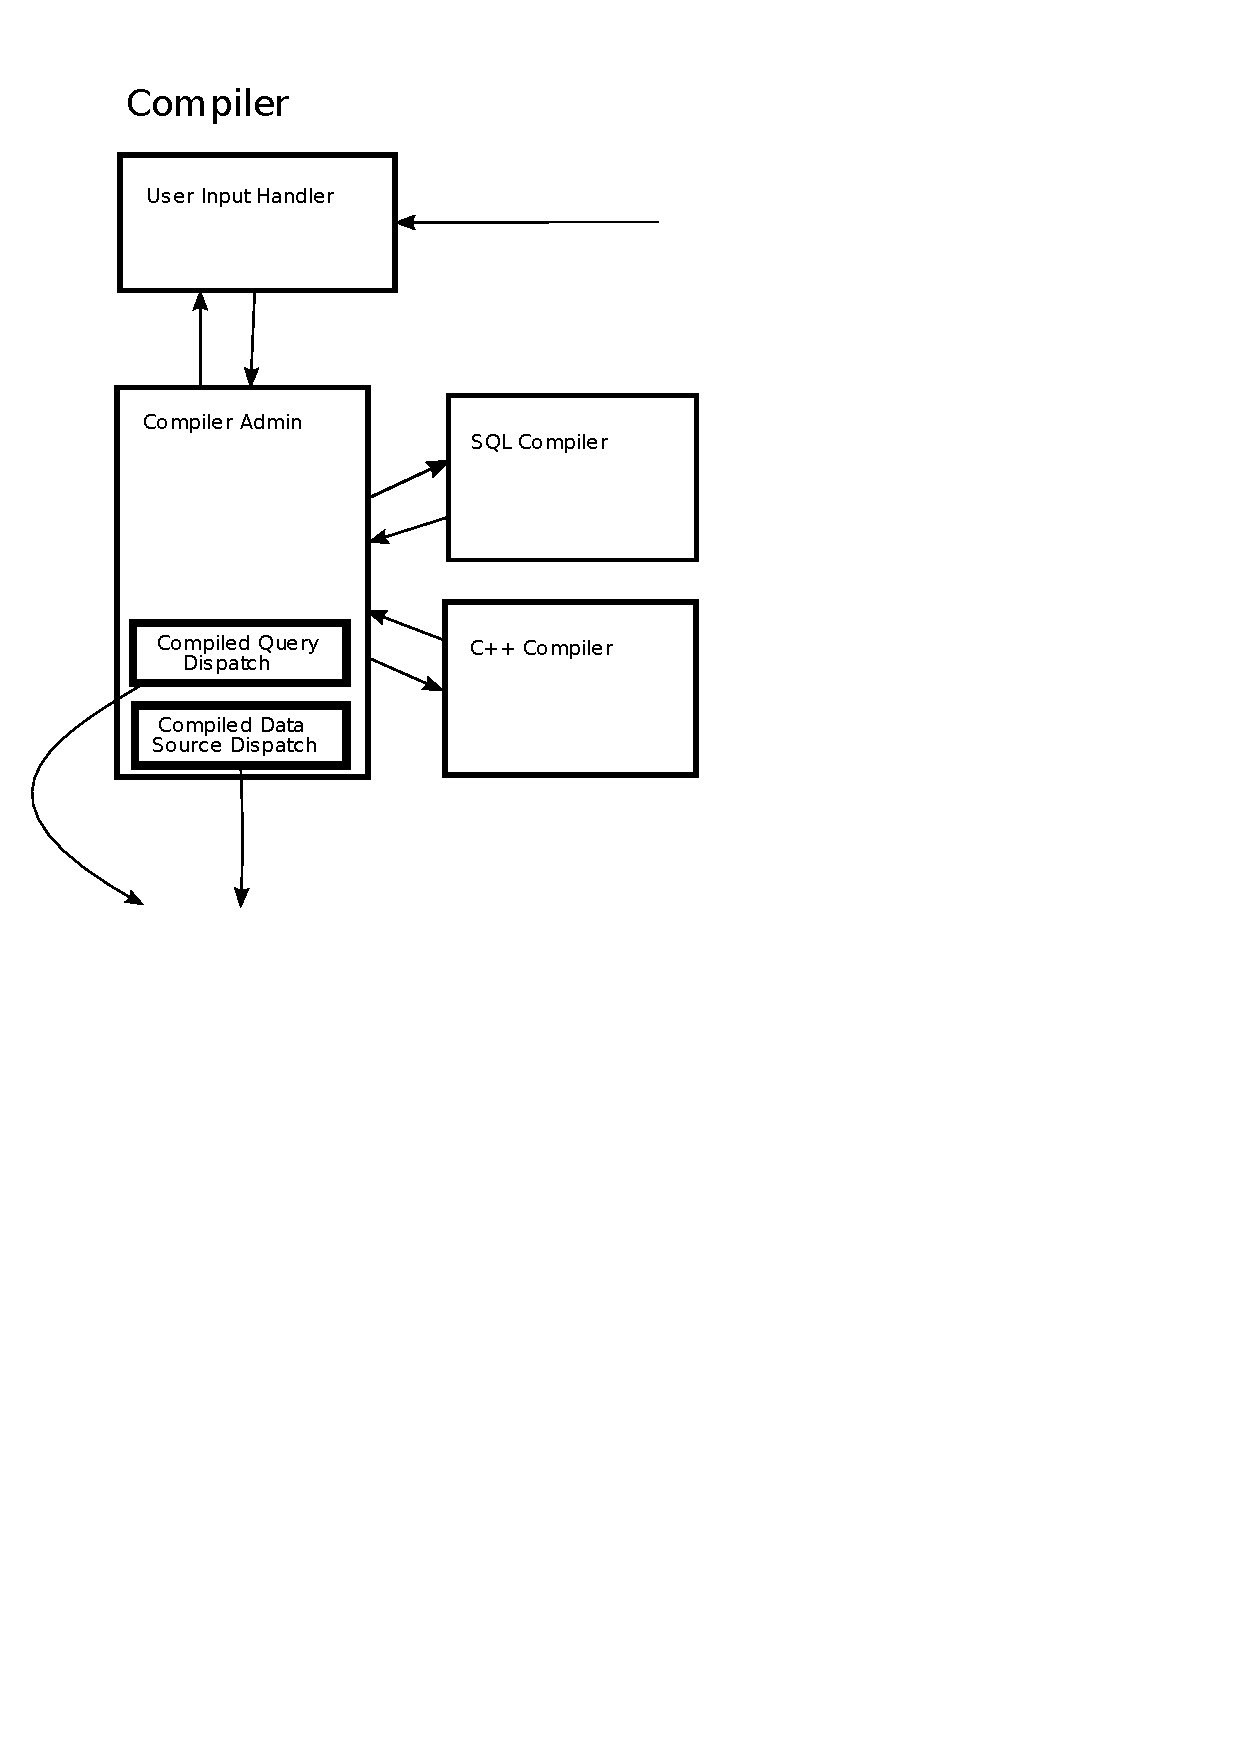
\includegraphics[width=4.50in]{figures/compiler.pdf}
  \caption{Wrapper Compiler Modules.}
  \label{fig:wrapper-compiler}
\end{figure}

\subsubsection{Example C++ code}
The C++ source code produced by the DBToaster compiler is a self-contained C++
source code file, that is it contains no references to external functions or
data structures with the exception of the C++ STL and Boost~\cite{url-boost}.
The C++ source code includes a set of map data structure and native type
variable definitions, as well as a set of event handling functions. As an
overview of our compilation process, the DBToaster compiler transforms SQL
queries defined over a set of input relations, to C++ functions that are capable
of computing a new query result given a delta, where deltas are an insertion,
deletion or update to a single relation. The DBToaster compiler produces a C++
function for each input relation used by the query, and we refer to these
functions as event handling functions. We show an outline of the C++ source code
below, for a SQL query using two relations \textit{bids, asks} as found in the
AlgoTrader application in Figure~\ref{fig:example-query-source}.

\begin{figure}[h]
\begin{Verbatim}
// Includes
#include <map>
#include <tuple>
#include <boost/any.hpp>
...

// Data structures
map<int, int> s_D_B;
map<tuple<int, int>, int> s_1_BC;
...

// Event handling functions.
// Arguments are relation's attributes.
void on_insert_bids(int t, int order_id, int p, int v) { ... }
void on_delete_bids(int t, int order_id, int p, int v) { ... }
void on_update_bids(int t, int order_id, int p, int v) { ... }

void on_insert_asks(int t, int order_id, int p, int v) { ... }
void on_delete_asks(int t, int order_id, int p, int v) { ... }
void on_update_asks(int t, int order_id, int p, int v) { ... }
\end{Verbatim}
\caption{Example query source code, compiled into an LLVM module.}
\label{fig:example-query-source}
\end{figure}

\subsubsection{Data Source and Adaptor Specifications}
The SQL queries specified to DBToaster include SQL data definition language
(DDL) extensions to support the specification of data sources. Currently
DBToaster provides two fundamental types of data sources: files and
sockets. Protocol-specific sources may be built on top of these primitive source
types, for example we could define a HTTP or Bluetooth source on top of a socket
source, and directly handle the protocol specification in a socket
adaptor.
\preliminary{We provide examples of DBToaster SQL statements for a CSV file and
network source in Figure~\ref{fig:source-sql-spec} (to be designed cleanly,
e.g. Figure~\ref{fig:source-sql-spec-redesigned}).}
\preliminary{(TODO: add an example of an adaptor specified as C++ code.)}

\begin{figure}[htbp]
\begin{Verbatim}[commandchars=\\\{\}]
-- Definitions of C types for tuples and adaptors
\preliminary{CREATE DATASET orderbook 'orderbook.h' 'adaptors.h'}

-- This example uses default values for ARGS, INSTANCE, ADAPTOR, BINDINGS
CREATE TABLE bids (
  t integer,
  order_id integer,
  price integer,
  volume integer
)
FROM '/home/yanif/datasets/orderbook/MSFT/20081201.csv'
SOURCE 'file'
TUPLE 'OrderbookTuple'

-- This example explicitly specifies ARGS, INSTANCE, ADAPTOR, BINDINGS
CREATE TABLE asks (
  t integer,
  order_id integer,
  price integer,
  volume integer
)
FROM '127.0.0.1:20000'
SOURCE 'network'
ARGS 'push'
INSTANCE 'asksSource'
TUPLE 'OrderbookTuple'
ADAPTOR 'OrderbookTupleAdaptor'
BINDINGS 't,t,order_id,order_id,price,p,volume,v'
\end{Verbatim}
\caption{Examples of data source specifications using DBToaster built-in sources and adaptors.}
\label{fig:source-sql-spec}
\end{figure}

\begin{figure}[htbp]
\begin{Verbatim}[commandchars=\\\{\}]
\preliminary{CREATE DATASET orderbook 'orderbook.h' 'adaptors.h'}

\preliminary{-- TODO: create and register sources/adaptors directly rather than inline}
\preliminary{CREATE ADAPTOR BidsAdaptor 'OrderbookTupleAdaptor'}

\preliminary{CREATE SOURCE BidsSource}
\preliminary{SOURCE 'network'}
\preliminary{FROM '127.0.0.1:20000'}
\preliminary{ARGS 'push'}
\preliminary{TUPLE 'OrderbookTuple'}
\preliminary{ADAPTOR BidsAdaptor}

\preliminary{CREATE TABLE bids (}
\preliminary{  t integer,}
\preliminary{  order_id integer,}
\preliminary{  price integer,}
\preliminary{  volume integer}
\preliminary{)}
\preliminary{FROM SOURCE BidsSource}
\preliminary{BINDINGS (}
\preliminary{  t t,}
\preliminary{  order_id order_id,}
\preliminary{  price p,}
\preliminary{  volume v}
\preliminary{)}
\end{Verbatim}
\caption{Example of possible redesign of source and adaptor specification.}
\label{fig:source-sql-spec-redesigned}
\end{figure}

\comment{
%% Anton's text.
Compiler consists of several components. Its structure can be seen in figure
\ref{CompilerPicture}. The main functionality of Compiler is to receive SQL
queries and Data Adaptors from users. When they are compiled, Compiler adds them
to Sources Processor or Query Processor respectively.

Two components responsible for compilation are SQL query pre-compiler and C++ code compiler. 

Compiler is an initial point of interaction with the DBToaster Runtime. Once
Runtime is up and running users initiate contact by specifying their need to
execute a query on some specific set of data sources or a desire to add an
update stream. User query and requests to add Data Adaptors are received by User
Input Handler. When Input Handler collects all needed informations, it is passed
to Compiler Admin. Compiler Admin converts SQL queries to C++ code and C++ code
to binary format. Compiled queries are passed to Query Admin to be added to a
list of actively executed queries. Data Source streams (Readers) are added by a
user providing a Data Adaptor for each stream. When Data Adaptor code is
compiled and user specified Reader is created, both are passed to Data Sources
Admin to be added to the list of active Readers. Reader and Adaptor for that
Reader form a pair where Reader receives data and Adaptor converts it to a
format understandable by Query Executor.

The Data Adapter is compiled into a binary format and sent to Data Sources Admin
to be added to Data Adaptors.
}

\comment{
\subsubsection{User Input Handler}
User Input Handler implements a server to handle client requests. Clients
connected to Input Handler Server send request types and parameters of that
request:
\\
\\
\begin{tabular}{|l|l|}
  \hline
  Type & Parameters \\ \hline
  Query & Query in SQL, list of Data Processor \\ \hline
  Reader & Connection Type, code for Data Adaptor \\ \hline
\end{tabular}
\\
\\
Thus User Input Handler responds to two type of requests one to add a SQL query
and another is to add Data Processor.
\\*
Add Query request requires the following information from users:

\begin{itemize}
	\item {\tt AddRequest(type="add query",\\
		 Source="SQL Source File",\\
	     DataReaders="list of Data Adaptors for this query");}
\end{itemize}

\noindent Add Data Stream request is as follows:

\begin{itemize}
	\item {\tt AddRequest(type="add stream", \\
	     AdaptorSource="C++ Adaptor Source file",\\
	     source="IPaddress and port or data input file");}
\end{itemize}

This information is forwarded to Compiler Admin:

\begin{itemize}
	\item {\tt Struct InputRequest( int type, string fileName,\\
	       list<int> informationSources \\
		   list<string> sourceParameters)}
\end{itemize}

User Input Handler serves as an interface for a server. Input Handler and
Compiler Admin are currently on the same execution path. In the future if needed
Compiler Admin can be separated to run in a different thread with the buffer to
store user requests from User Input Handler.
}

\subsubsection{Compiler Admin}
The Compiler Admin provides the following interface to enable clients to submit queries.

\begin{Verbatim}
string runQuery(string sqlText, list<string> adaptorCode);
\end{Verbatim}

This method accepts the contents of a SQL file as a string, and a set of
adaptors written in C++, writes these files out to a temporary file for
compilation, registers adaptors as necessary, and the invokes the two phases of
compilation.

This method returns the status of the compilation process, specifically any
compilation errors that may have occurred during either the SQL compilation
phase, or the C++ compilation phase. The DBToaster compiler should not expose
low-level C++ compilation errors specific to our compilation process to the
user, rather should be able to identify a high-level SQL statement, a source
name, or an adaptor specification statement where the error lies.

\preliminary{
Registering an adaptor involves placing the adaptor code in a local adaptor
repository maintained in the DBToaster Server's catalogs, and tracking the
association of the adaptor name and the adaptor code file. This enables one-time
specification of an adaptor, and subsequent reuse of that adaptor across
multiple sources (e.g. one adaptor for multiple network connections such as a
sensor data adaptor, used to handle 100 sensors' input streams). We return to
this when describing the catalog data structure as part of the Query Processor.
}

\preliminary{For a single-node server, this method may be exposed to DBToaster
clients via an XML-RPC interface, or by a custom protocol with access provided
by a client library that can be embedded into application code (e.g. like JDBC
driver files). For the distributed setting it is likely that we will not want to
provide direct access to computation servers, rather this interface would be
provided by a proxy or frontend to the DBToaster Server Farm.}

\preliminary{For the time being, compilation requests are handled in serial
fashion since we anticipate a low volume of queries being submitted to the
system at any point in time, and a low overhead compilation process. This may be
changed to either an event-handling, or thread pool model at a future stage as
needed based on revised assumptions of either the query submission model or with
a higher overhead compiler.}

In addition to the SQL and C++ compiler interfaces which we describe below, the
Compiler Admin assumes the following interfaces from the catalog, Data Sources
Processor and Query Processor:

\begin{Verbatim}
status Catalog::registerAdaptor(AdaptorId adaptorId);
status DataSourceAdmin::runSourceAndAdaptor(
    map<SourceId, AdaptorId> sourcesAndAdaptors);
status QueryAdmin::runQuery(
    queryId, list<HandlerId> handlerIds, list<SourceId> sourceIds);
\end{Verbatim}


%%
\comment{
Compiler Admin takes source code from User Input Hander, compiles it to
executable code and dispatches it to either Data Sources or Query Processor.
\comment{
Once user request is received, Compiler Admin takes over. Depending on the type
of the request Admin takes different actions.
}

On SQL query request Admin passes SQL query source file to SQL Compiler. SQL
compiler returns a file containing C++ implementation of it. This file is passed
to C++ compiler. C++ compiler returns a function handle to compiled binary of
this query. Finally query handle is passed to Query Admin to be added to a list
of executable queries.

On Reader request Admin passes Data Adaptor file to C++ compiler, which returns
a function handle to Data Adaptor. Admin creates a Data Source Reader and opens
a connection (either a socket or a file). Handle to Data Source together with
handle to Data Adaptor is passed to Data Sources Admin.
}
%%

\noindent An outline of the Compiler Admin class is as follows:
\begin{Verbatim}
class CompilerAdmin
{
public:
    void runQuery(string sqlText);

private:
    struct ModuleIds {
        QueryId queryId;
        list<HandlerId> handlerIds;
    };

    FileName  compileSQL(string sqlFileName);
    ModuleIds compileCPP(string cppFileName);
	
    SQLCompiler       dbtoaster;
    CCompiler         cc;
    Catalog*          serverCatalog;
    QueryAdmin*       queryAdmin;
    DataSourcesAdmin* dsAdmin;
}
\end{Verbatim}

The method \texttt{runQuery(sqlText)} takes a query execution request specified by
\texttt{sqlText}. The Compiler Admin contains instances of a SQL Compiler and C++
Compiler. It also has access to the Catalog, and Query Admin and Data Sources
Admin subcomponents of the Query Processor and Data Source Processor
respecitvely to initialize queries, sources and adaptors.

\subsubsection{SQL Compiler Interface}

We now outline the implementation of the following method:

\begin{Verbatim}
FileName compileSQL(string sqlFileName);
\end{Verbatim}

The DBToaster Wrapper Compiler invokes the SQL compiler (the \texttt{dbtoaster}
binary) as a new process through the \texttt{system()} syscall.  We refer the
user to the \texttt{dbtoaster} manual and the source code for more information
regarding the arguments passed to \texttt{dbtoaster}. The compiler generates a
C++ source code file named the same as the temporary SQL query file with a
\texttt{.cpp} suffix in the query repository directory specified as part of the
server's configuration file. The compiler also generates a query manifest file
(with a \texttt{.dbtmf} extension) listing all handler functions and any
additional library dependencies of the compiled code.
\preliminary{Additionally the compiler produces compilation logs and analysis
  traces from the query compilation process that may be used by the optimizer.}
\preliminary{As future work, \texttt{dbtoaster} could expose a programmatic
interface to support compilation, enabling the Wrapper Compiler to directly
perform compilation and retrieval of analysis traces.}

\comment{
The SQL compiler takes SQL query from a file and creates an optimized, DBToaster,
C++ coded to be added to the runtime. File containing code is returned to the
Admin.
}

\subsubsection{C++ Compiler Interface}

The following method implements C++ compilation:

\begin{Verbatim}
ModuleIds compileCPP(string cppFileName);
\end{Verbatim}

This method invokes the C++ compiler (\texttt{llvm-g++}) also through a
\texttt{system()} syscall. We use the LLVM C++ compiler to produce LLVM bitcode
(as opposed to LLVM machine code), subsequently invoking JIT compilation on the
bitcode prior to execution inside the Query Processor. This enables easier
introspection of the compiled code using LLVM and its tools.  Our C++
compilation method returns a new identifier for the query as a whole, as well as
individual identifiers for each handler function through the \texttt{ModuleIds}
structure.

\comment{
C++ compiler takes file containing C++ code. It builds binary code, loads it in
memory and returns a function handle to it to Admin.
}

\subsection{Data Source Processor}

The Data Source Processor receives updates from the various streams supplied to
or requested by queries running at the server. 
For a fully extensible data source model, we assume each Source is associated
with two function pointers, determined by the Compiler Admin: a Source function,
for reading data that returns raw bytes, and an Adaptor function for
transforming the raw bytes into a structured tuple.
\preliminary{The functions themselves are maintained in a Source and Adaptor
Repository in the server's Catalog data structure, and referenced by their
SourceId and AdaptorId. We assume the functions are initialized during the
compilation process.}
\preliminary{Source functions performs low-level reading from the associated
file descriptor.  using the C++ STL to handle file inputs, and Boost to read
from sockets.}
Each Source function is pushed onto a Runable Sources Queue, and receives data
from outside streams and forwards tuples received to a Data Dispatcher.

Each Adaptor function is registered with the Data Dispatcher. Adaptor functions
format, transform and manipulate the raw bytes read to produced a structured
tuple for query processing. Currently our adaptors assume as one-to-zero or
one-to-one model of tuple processing -- that is each adaptor must produce zero
or one tuple from its work.  Following tuple adaption, the tuple is passed to
the Input Buffer component of the Query Executor, where it is queued for
processing until the relevant query is next scheduled.
\preliminary{This model may be revisited and generalized in the future to
support one-to-many tuple adaption, which in turn will require changes in the
interaction between the Adaptor and Input Buffer subcomponent of the Query
Processor}.

The execution model for the Data Source Processor is also based on a
multi-threaded paradigm, backed by a thread pool, and a set of pending sources
maintained in the Runable Sources Queue. Each worker thread

\begin{itemize}
\item Picks a Source function from the Runnable Sources Queue.
\item Performs a data read by invoking the Source function.
\item Forwards read data tuple to Data Dispatcher, which subsequently invokes an
  associated Adaptor function.
\end{itemize}

\noindent We present a detailed representation of the Data Sources Processor in
Figure~\ref{fig:data-source-proc}.

\comment{
where each thread picks a Data Reader and executes a read at a time from one of
them. Once read is done the results of the read are forwarded to a Data
Structure Dispatch. The Dispatch uses the appropriate Data Adapter to handle the
data into a structured format, then the structured data is forwarded to Query
Processor, in particular to the Query Tuple Queue. The more pictorial
description can be found in figure \ref{fig:data-source-proc}.
}

\comment{
processing consists of the list of list of stream points. Each point is given by
the user and signifies a way for a DBToaster to connect with the input stream of
some process which dispatches data to the DBToaster. Each Stream Point is
written by the user and user can fully specify how the data should be received
and processed. Stream point is responsible for sending data to the Data Dispatch
unite in a pre-specified format. The structure for data source processing can be
found in figure
}

\begin{figure}
  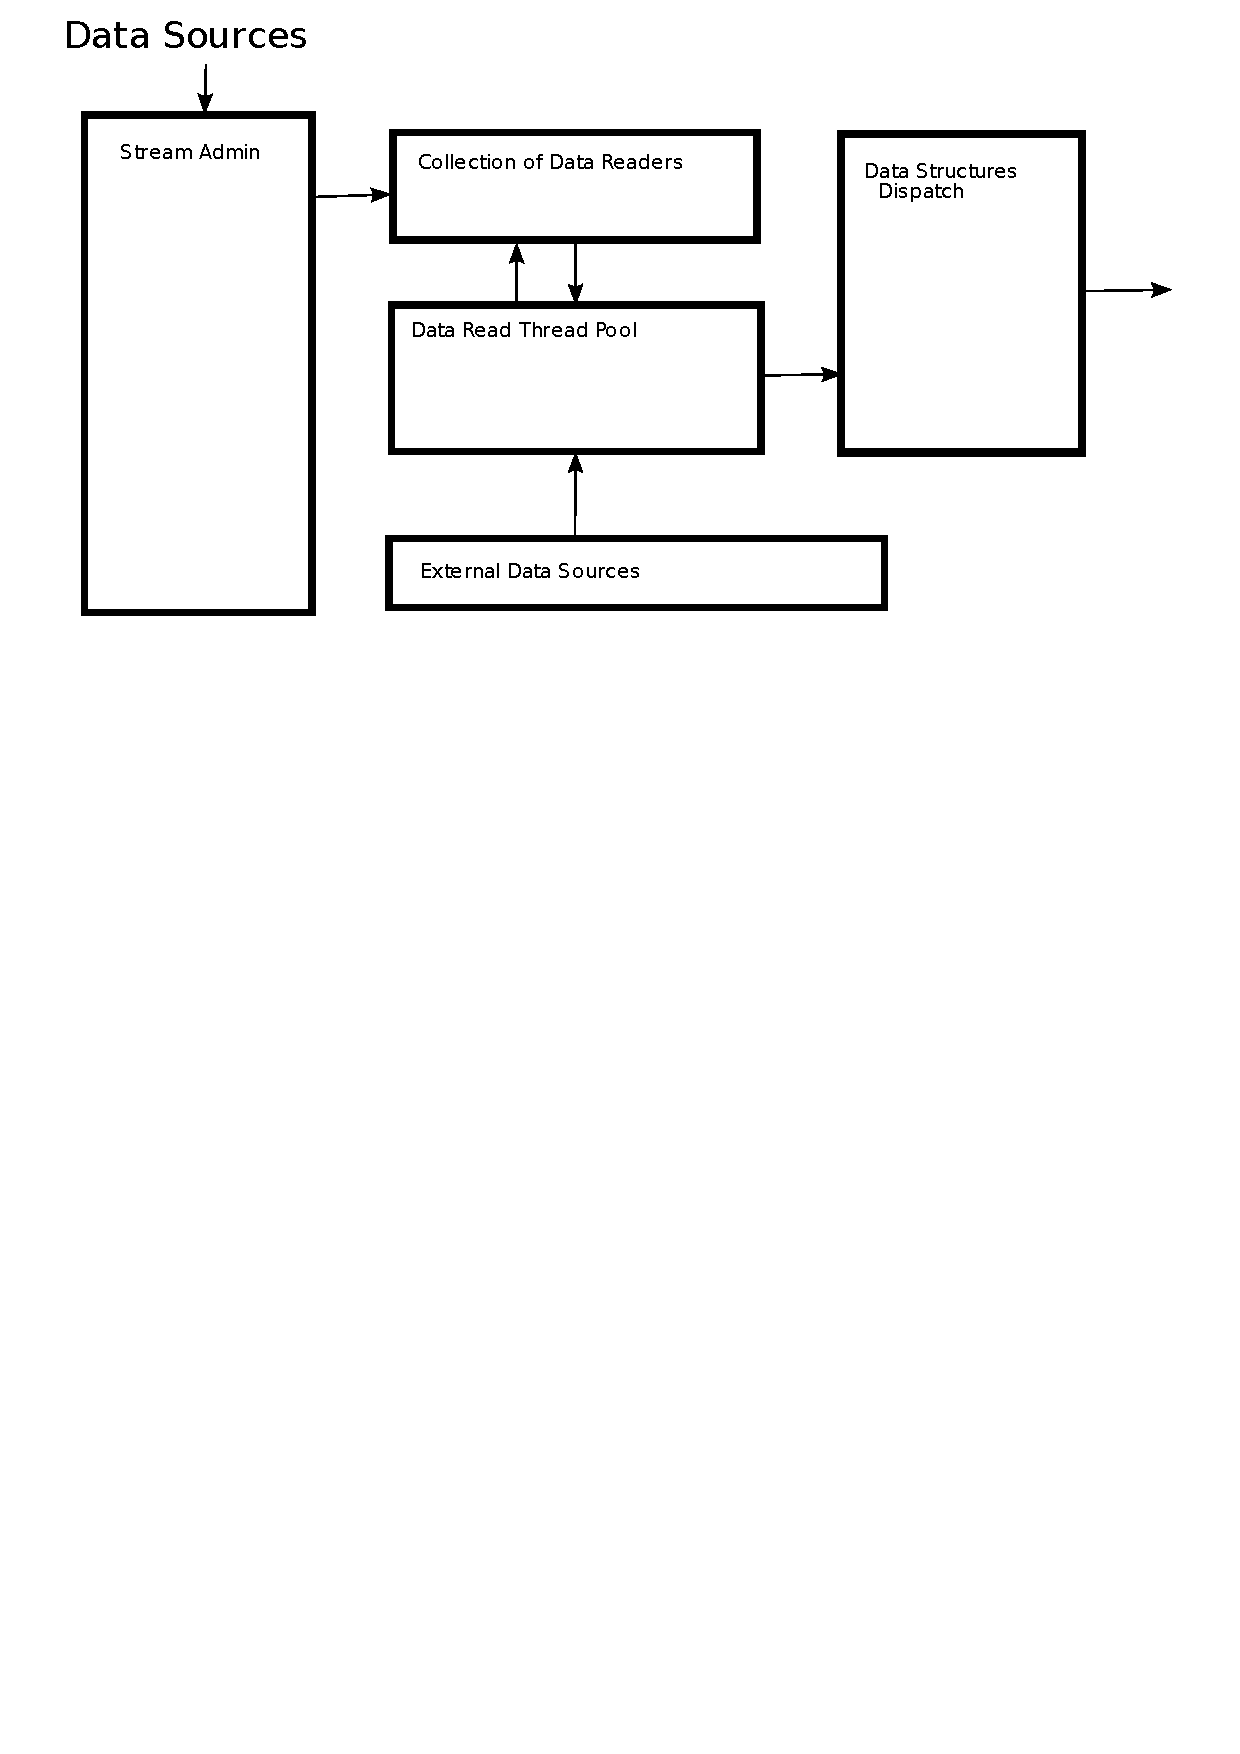
\includegraphics[width=5.00in]{figures/DataSources.pdf}
  \caption{An overview of the Data Source Processor.}
  \label{fig:data-source-proc}
\end{figure}

\subsubsection{Data Sources Admin}

The Data Source Processor Admin provides the control interface for the Data
Source Processor. Currently this consists of methods to deploy and remove
sources from feeding data to the Query Processor. The Data Source Admin houses
both the thread pool for running Source functions and the Data Dispatcher, which
evaluates the Adaptor functions and forwards the new tuples to the Query
Processor.
In addition the Data Source Admin has a reference to the InputBuffer.
The InputBuffer is a multi-queue data structure which buffers tuples for
processing in the Query Executor to support concurrent execution of queries
while preserving the order in which tuples are processed by each query. We
describe our concurrency model in greater detail when describing our Query
Executor. The Data Source Admin expects the following methods to be present in
the InputBuffer:

\begin{Verbatim}
void InputBuffer::addTuple(SourceId, void* structuredTuple);
\end{Verbatim}

\comment{
Data Sources Admin provides an interface for adding new Data Sources. Each Data
Source is paired up with a Data Adaptor. The later converts raw data tuples to
format understood by query.

Another reason for Data Sources Admin is to provide a level of abstraction since
calls for Data Source and Data Adaptor additions will be executed in the
compiler execution path.
}

\noindent Finally, we outline the Data Source Admin class below:

\begin{Verbatim}
class DataSourceAdmin
{
public:
    DataSourceAdmin(InputBuffer*, Catalog*);
    runSourceAndAdaptor(map<SourceId, AdaptorId> sourcesAndAdaptors);

private:
    Catalog*       catalog;
    DataSourcePool sources;
    DataDispatcher dispatcher;
    InputBuffer*   tupleBuffer;
}
\end{Verbatim}

\comment{
\noindent Data Source Admin is also responsible for handling Data Dispatcher and
Data Sources Manager.
}


\comment{
Data Sources Admin receives two function handles one to a data Reader and
another one for a Data Adaptor from a Compiler. First Admin locks Data Adaptors
and inserts a new Data Adaptor. Then Admin locks Data Readers Queue and a handle
is inserted. Each Data Readers handle implements a method \emph{readNext()} for
reading data from some data source (typically a socket or a file).

\begin{itemize}
	\item {\tt rawDataTuple getNext(); // user defined function - provided}
\end{itemize}

\noindent The {\tt rawDataTuple} is a pair {\tt <size, bit-string>}.

The Reader extracts the informations from either a file or a socket. Reader's
communication with the outside world is in a standard format. On a read request,
Reader first reads a header containing the information about the message
followed by the message itself. For now we assume that a header is an integer
containing the number of byte to be read. Once the read is completed the size
and message are forwarded to Data Structures Dispatch.

%\noindent Data Sources Admin class contains the following:
}


\subsubsection{Data Source Pool}

The Data Source Pool contains a list of worker threads, and provides standard
thread pool functionality of maintaining a queue of jobs (in this case Source
functions to perform reads), that can be added to or removed from in a
concurrent manner. Each worker thread performs the following tasks during its
lifetime:
\begin{itemize}
\item gets a Source function from the runnable source queue.
\item reads a raw input tuple with the \texttt{readNext()} method.
\item forwards the resulting \texttt{rawDataTuple} to the Data Dispatcher along
  with a SourceId.
\end{itemize}

\noindent Each worker thread assumes the following interface from the Data
Dispatcher, to invoke an Adaptor function:

\begin{Verbatim}
    void dispatchNext(SourceId, RawDataTuple);
\end{Verbatim}

\noindent The Data Source Pool is defined as follows:

\begin{Verbatim}
class DataSourcePool
{
public:
    void run();

private:
    list<thread>            runningThreads;
    DataSourceQueue         runnableSourceQueue;
    DataDispatcher*         dispatcher;
}
\end{Verbatim}

\noindent It contains a Data Source Queue, which is essentially a concurrent queue:

\begin{Verbatim}
class DataSourceQueue
{
public:
    FunctionHandle  getSource();
    void            putSource(FunctionHandle);

private:
    queue<FunctionHandle>  sources;
}
\end{Verbatim}

\noindent and a pointer to the Data Dispatcher.

\subsubsection{Data Dispatcher and Structured Tuples}

The Data Dispatcher receives a SourceId identifying a Source with a new input
tuple, as well as the raw tuple read by that Source.

\comment{
\begin{itemize}
\item {\tt dispatchNext(readerID, rawDataTuple);}
\end{itemize}
}

Based on the SourceId, the Data Dispatcher calls an appropriate Adaptor function
to convert incoming {\tt RawDataTuple} message into a structured message that
can be handled by queries running in the executor. The structured tuple is then sent
to an appropriate set of queues in the Input Buffer. The DBToaster Server
internally represents such structured tuples with the \texttt{StructuredTuple}
class, and conceptually this is a pair containing the tuple size and a bit
sequence representing tuple fields (i.e. \texttt{pair<size\_t, string>}). Note
that we adopt a black-box approach to the format of the structured tuple within
the scope of the Data Source Processor, since we do not need to distinguish any
particular field within the tuple during the Data Source Processor's work. The
format assumed by the Query Processor however is that this bit sequence
represents a packed binary struct (i.e. a C-struct defined with the
\texttt{\_\_packed\_\_} attribute).

\noindent The Data Dispatcher is outlined below:

\begin{Verbatim}
class DataDispatcher
{
public:
    void dispatchNext(SourceId, RawDataTuple);

private:
    void sendData();

    DataAdaptors adaptors;
    InputBuffer* tupleBuffer;
}
\end{Verbatim}

\noindent The DataAdaptors class is a map enabling access to the appropriate
Adaptor function for a given Data Source.

\begin{Verbatim}
class DataAdaptors
{
public:
    FunctionHandle  getAdaptor(sourceID);
    void            putAdaptor(sourceID, FunctionHandle);

private:
    map<sourceID, FunctionHandle> adaptorFunctions;
}
\end{Verbatim}

\subsection{Query Processor}

The bulk of the query processing work is done by the Query Executor component,
which includes a Scheduler component that executes queries using a thread pool
model, with worker threads denoted as Query Threads. As data is enqueued in the
InputBuffer by the Data Dispatcher, the Scheduler is notified of a new job,
which in turn makes the associated query available for execution by adding the
query to the runnable query queue as necessary. Our scheduler is currently a
simple round-robin scheduler in terms of available jobs, and simply picks the
first runnable query and hands this to a Query Thread for execution. Each Query
Thread picks a query-tuple pair from the InputBuffer and processes it. The
structure of query processor can be found in figure \ref{fig:query-processor}.

\begin{figure}
  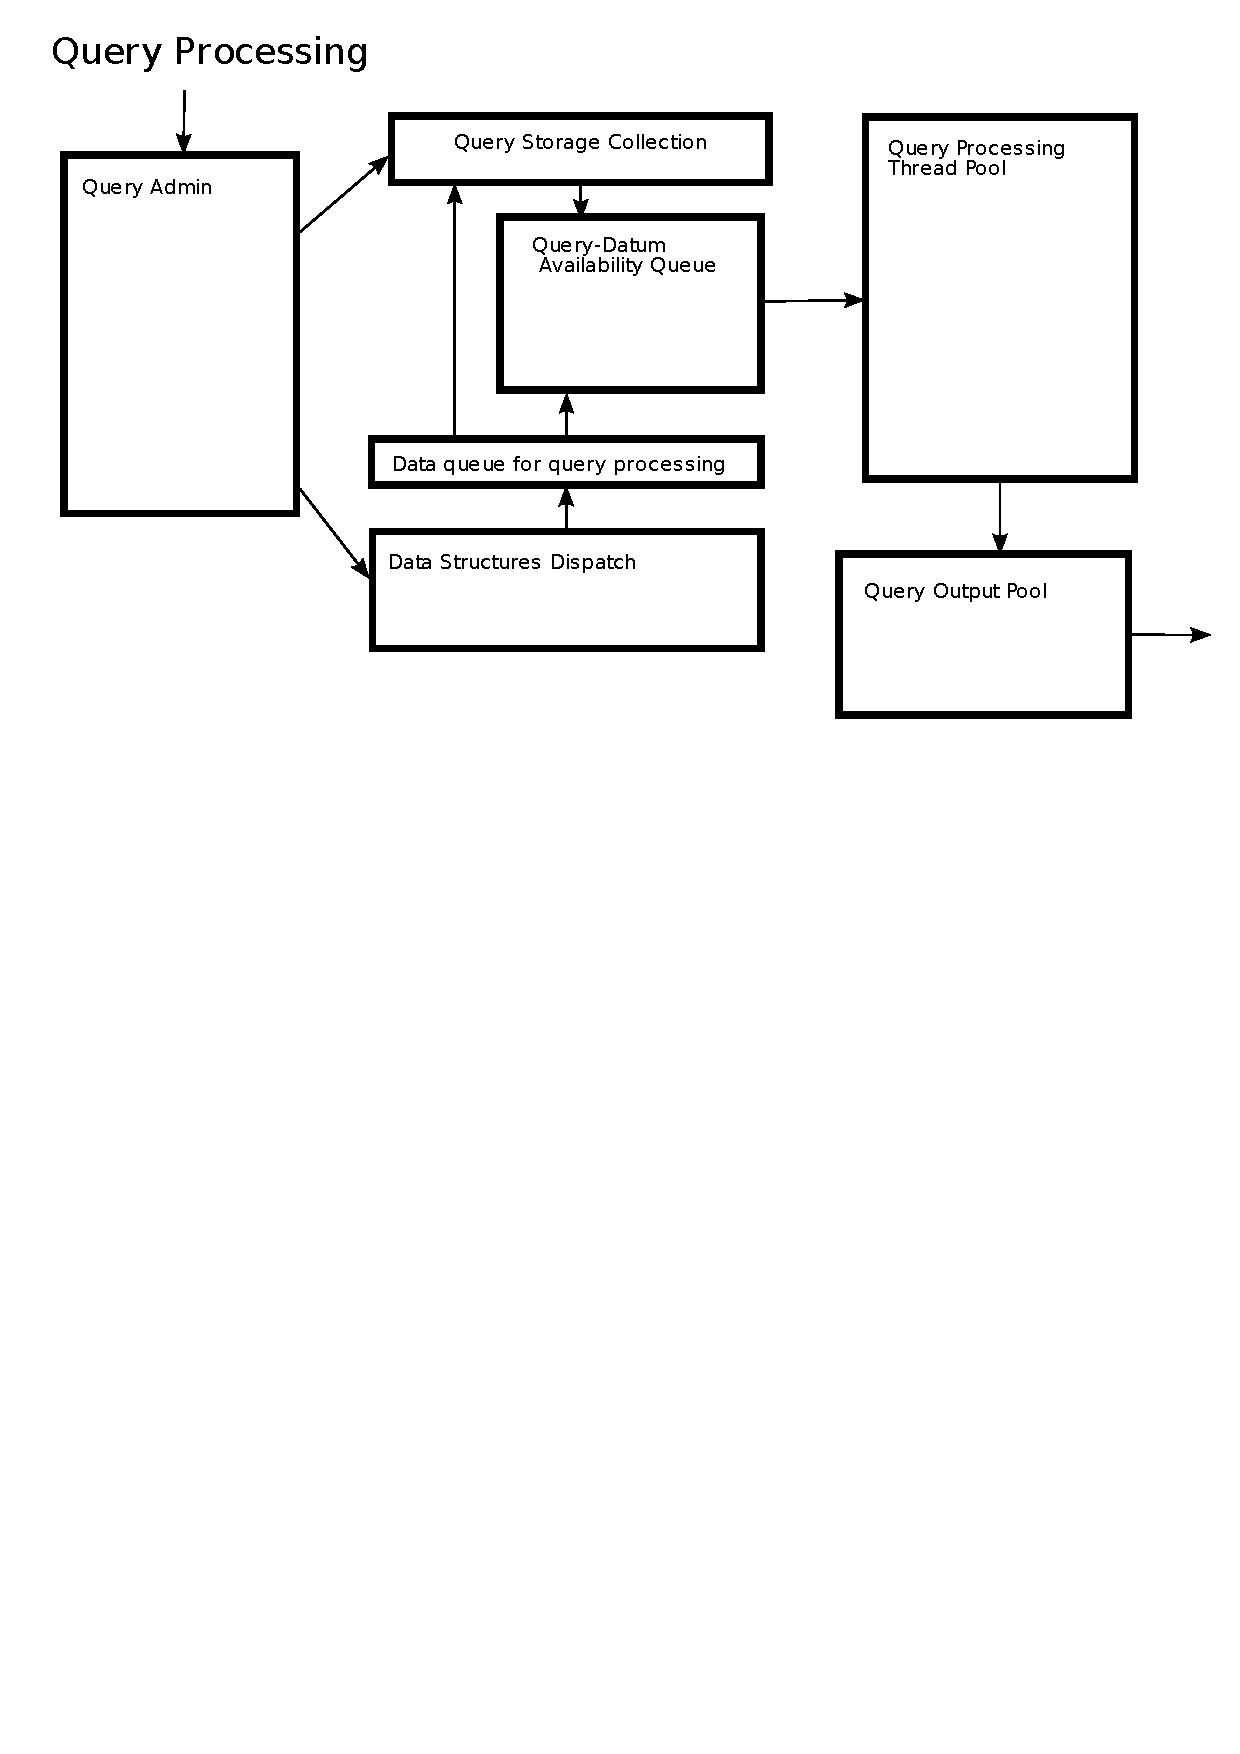
\includegraphics[width=5.00in]{figures/QueryProcessing.pdf}
  \caption{Query Processing Management.}
  \label{fig:query-processor}
\end{figure}

\subsubsection{Query Admin}

The Query Admin receives a function handle for a query. It also receives a list
of SourceIds which provide data for that query. When the query's function handle
is received, the Query Admin locks the Catalog and inserts the query handle
there. After that, the Query Result Queue is locked and updated to create an
output queue for the new query. Finally the Query Admin locks the InputBuffer
and adds a new queue to buffer arriving data intended to be processed by the new
query.

The Catalog contains a map to track queries and their associated function handles. 
\preliminary{(TODO: describe Catalog class.)}
The Query Admin class is designed as follows:
\begin{Verbatim}
class QueryAdmin
{
public:
    runQuery(QueryID, FunctionHandle, list<SourceId> querySources);

private:
    Catalog      catalog;
    InputBuffer* tupleBuffer;
}
\end{Verbatim}


\subsubsection{Query Executor}

The Query Executor consists of two interdependent components: Input Buffer and
Scheduler. The Input Buffer stores data needed for query execution. The
Scheduler maintains a thread pool. Each thread runs one query at a time using
one update tuple from the Input Buffer. \emph{InputBufferInterface} and
\emph{SchedulerInterface} are two classes providing interfaces for
\emph{InputBuffer} and \emph{Scheduler}.

\paragraph{Input Buffer.}

The Input Buffer provides in-memory storage of pending tuples waiting for
processing. It contains a queue per data source. Each query needs to register
with the Input Buffer to access data from it. The Input Buffer receives a new
tuple from Data Dispatcher with a SourceID (in the format of a {\tt
StructuredTuple}), and inserts the new tuple into the appropriate queue. If a
tuple insert causes the query to become available, the Scheduler is notified to
add the query for processing. If a query is already runnable, the new tuple is
simply inserted into the appropriate queue without any action.

\noindent The \texttt{InputBufferInterface} has the following structure:

\begin{Verbatim}
class InputBufferInterface
{
    void    addTuple(SourceID, StructuredTuple);
    void*   getTuples(QueryID);
    void    addQuery(QueryID, SourceID);
    void    removeQuery(QueryID);
    void    hasNext(QueryID);
    void    removeTuples(QueryID);
}
\end{Verbatim}

\noindent The \texttt{InputBuffer} class has the following structure:

\begin{Verbatim}
class InputBuffer
{
public:
    InputBuffer(MemoryManager*);
    void    addTuple(SourceID, StructuredTuple);
    void*   getTuples(QueryID);
    void    addQuery(QueryID, SourceID);
    void    removeQuery(QueryID);
    void    hasNext(QueryID);
    void    removeTuples(QueryID);
    void    addScheduler(SchedulerInterface*);

private:
    MemoryManager*                     mm;
    Scheduler*                         schedulingQueue;
    map<SourceID, list<TupleQueue*> >  sourceAccess;
    map<QueryID,  list<TupleQueue*> >  queryAccess;
    map<SourceID, list<QueryID> >      availableQueries;
}
\end{Verbatim}

\noindent Here we refer to {\tt QueryID} as an ID of a query, which needs data
from a particular data source. This ID is created by the Catalog when a query is
added to it. Its purpose is to support an association between a query and a
source. It encapsulates the details of dealing with several sources for each
query inside the Scheduler.

The interface function {\tt addTuple(SourceID, StructuredTuple)} is called by
the Data Dispatcher to add a new data item. The functions
\texttt{getTuple(QueryID)}, \texttt{hasNext(QueryID)} and
\texttt{removeTuples(QueryID)} are required to extract tuples available for the
query to be executed as well as for cleaning up queues. Functions {\tt
addQuery(QueryID, SourceID)} and {\tt removeQuery(QueryID)} are needed by Query
Admin to insert or remove a new queries.

To enable this functionality we need to consider concurrency and efficiency. 

\subparagraph{Concurrency:} Each queue can be accessed by several queries. Also
each queue has only one data source associated with it. The queue is locked on
insertion and deletion from the Data Dispatcher. Data reads are enabled to all
queries simultaneously. \emph{SharedTupleQueue} provides these controls
internally for each queue. Since there is no interaction between different
queues there is no need to manage concurrency issues between them.

\subparagraph{Efficiency:} The main inefficiency comes from the fact that data
from one data source needs to be accessed by several queries. If we adopt a
simple model (referred to as \textit{disjoint} queueing), each query has its own
set of queues for each source. Here we have the inefficiency of copying data to
each such queue. The benefit of such model is its simplicity of implementation
and use, the obviation of concurrency management mechanisms. Another model
(\textit{shared} queueing) is to have only one queue for each data source that
is shared by all queries using the source. In this case each queue will need to
keep track of which query requires what data item from this queue. Removing
queued tuples becomes complicated. The benefit of this method is a lower
overhead storage method and memory management. Both approaches can be
supported. We can hide all details into the implementation of queue and Input
Buffer. By requiring the following specification:

\noindent In disjoint queueing, we define the Tuple Queue data structure as:
\begin{Verbatim}
class QueryTupleQueue
{
public:
    QueryTupleQueue(MemoryManager*);
	
    void    addTuple(structuredTuple);
    void*   getTuples();
    bool    isEmpty();

private:
    queue<StructuredTuple>   tuples;
}
\end{Verbatim}

\noindent For shared queueing, we define the Tuple Queue data structure as:
\begin{Verbatim}
class SharedTupleQueue
{
public:
    SharedTupleQueue(QueryID, MemoryManager*);

    TupleQueue*       join(QueryID);
    void              removeQuery(QueryID);

    void              addTuple(StructuredTuple);
    StructuredTuple   getTuples(QueryID);
    bool              isEmpty(QueryID);
    void              removeTuples(QueryID);

private:
    map<QueryID, PointerToPositionInQueue>     nextTuple;
    queue<SharedTuple>                         tuples;
    MemoryManager*                             mm;
}
\end{Verbatim}

\begin{Verbatim}
struct SharedTuple
{
    int               beenAccessed;
    StructuredTuple*  tuple;
}
\end{Verbatim}

In the current implementation we have adopted shared queueing due to memory
savings and the efficiency of data copying.

When a new query is inserted into Query Admin, Input Buffer is called with {\tt
addQuery(QueryID, SourceID)} for each data source (remember that QueryID is an
ID indicating query-source associations and is mapped to an actual query in the
Catalog). If a source is not present (we can check for it through our {\tt
map<SourceID, list<TupleQuery*> >}), we create a new Tuple Queue. If it is
present, we call {\tt join(QueryID)}. In disjoint queueing, the method {\tt
join(QueryID)} creates a new TupleQueue and returns a pointer to it. With shared
queueing, it will return a pointer to this queue and change the internal
structure to accommodate a new query. (The method {\tt removeQuery(queryID)}
applies the reverse -- it either removes a queue or changes internal
representation). New tuples are added by the call of {\tt addTuple(SourceID,
StructuredTuple)} in \emph{InputBuffer} from Data Dispatcher.

\subparagraph{Memory Manager.} The Memory Manager facilitates storage of data
tuples by pre-allocating a number of pages. The Memory Manager provides an
interface for allocating and deallocating space for data by allocating a set of
new pages and deallocating unused pages.

\begin{Verbatim}
class MemoryManager
{
    void*  getPage();
    void   returnPage();
}
\end{Verbatim}

\noindent To ease the management of page memory, we define the class Page
Manager. It keeps track of all relevant information needed to allocate space for
new tuples.

\begin{Verbatim}
class PageManager
{
    PageManager(MemoryManager*);
    void*  getSpace(int* size);
    void   free(void* position, int* size);
}
\end{Verbatim}

\paragraph{Scheduler}

The Scheduler's job is to execute a query on any pending data tuple. To enable
concurrent execution of queries, especially with today's multicore
architectures, we adopt a thread pool model for executing queries. Each thread
is responsible for picking up a query from a RunnableQueryQueue. Then thread
runs a query on data tuple retrieved from the Input Buffer. Results are put into
a Query Results Queue. Results are accessed by users upon request.

\noindent The execution flow within each thread is as follows:

\begin{algorithm}
\caption{QueryThread::run()}
\begin{algorithmic}
\LOOP
    \STATE get a QueryID from the RunnableQueryQueue
    \STATE get a set of data tuples from the Input Buffer
    \STATE get a query function handle from the Catalog
    \STATE run the query function on the data tuples
    \STATE remove the data tuples from the InputBuffer
    \IF {more tuples are available for this query}
        \STATE put query onto RunnableQueryQueue
    \ENDIF
    \STATE put results to QueryResultsQueue
\ENDLOOP
\end{algorithmic}
\end{algorithm}

\noindent The Scheduler class contains the following:

\begin{Verbatim}
class Scheduler
{
public:
    Scheduler(QueryCatalog*);
    void run();
    void addRunnableQuery(querySourceID);

private:
    RunnableQueryQueue   availableQueries;
    list<thread>         executionThreads;
    InputBuffer*         readyData;
    QueryCatalog*        queryHandles;
}
\end{Verbatim}

Function {\tt addRunnableQuery(querySourceID)} is used by the Input Buffer to check
if current query is available for execution. If query is not available, it is added
to the RunnableQueryQueue.

\noindent We define the RunnableQueryQueue class as follows:

\begin{Verbatim}
class RunnableQueryQueue
{
public:
    QueryId nextQuery();
    void    addQuery(QueryID);
    void    removeQuery(QueryID);
    bool    isActive(QueryID);

private:
    queue<QueryID>    readyQueries;
}
\end{Verbatim}


\subsubsection{Query Results Queue}

\preliminary{
The Query Results Queue implements a staging area for query results, where each
client upon connection indicates a set of queries they are interested in.
}

\begin{itemize}
\item {\tt userDataStructuresDispatch(UserID, Query ID list);}
\end{itemize}

\noindent The DBToaster Server maintains a map of query IDs to a queue of query
results to be sent to each client. When a query produces an output, it is sent
to Query Result Queues, where query results are buffered until requested by
clients.

\begin{itemize}
\item {\tt queryDataStructuresDispatch(QueryID, QueryMap);}
\end{itemize}

\noindent When a client needs a new piece of information it sends a request to
server with query ID and number of tuples needed.  The DBToaster Server returns
results of that query.

The Query Result Queue implements two ways to access data. In the first one a user
asks for a complete query result. In the second one user asks for a cursor to
query results and is capable of iterating over results.

The Query Result Queue class is defined as:

\begin{Verbatim}
class SchedulingQueue
{
public:
    getFullQueryResult(ClientID, QueryID);
    startCursorResult(ClientID, QueryID);

private:
    map<queryID, queryResult> pendingResultsMap;
}
\end{Verbatim}








\section{AlgoTrader}

AlgoTrader is an application that applies DBToaster Runtime to a domain of Stock
Exchange and Algorithmic Trading. It consists of two parts: an automatic Stock
Trading Simulator and a platform for development and execution of Automatic
Stock Trading Algorithms. The purpose of AlgoTrader is to demonstrate the
potential of DBToaster Runtime to process time critical, expressive queries over
streaming data. To demonstrate the potential of Runtime two components are
needed: a source(s) of update stream and an application(s), which runs queries
over it. Exchange Server Simulator provides a source of continuous stock
transactions between interested parties. AlgoEngine implements a set of trading
strategies. Each strategy utilizes results of a query over the data from
Exchange Server Simulator to make a decision about purchase/sell of
stocks. Queries are processed and executed by DBToaster Runtime.
  

\subsection{Exchange Server Simulator}
Exchange Server Simulator (ESS) is designed to reproduce the behavior of
Electronic Communication Networks (ECN). ECN facilitates stock exchanges between
different parties connected to the network. Each ECN provides certain data to
its subscribers. For now we limit ourselves to complete knowledge about changes
in stock order books. Order books for a stock contains all sell (ask) and buy
(bid) request for each stock. This data is distributed to all subscribers as a
constant stream of updates to order books. Current implementation of Exchange
Server Simulator works with only one stock (for now).

Each Order Book consists of an Asks Book and Bids Book. Asks Book contains sell
requests, Bids Book - buy requests. Each ask/bid request is transmitted to all
subscribers. If two requests are matched the results of such a match are
transmitted as well.

Main difference between a real ECN and a Simulator, is simulator's ability to
replay the exchanges made at some earlier date and incorporate exchanges made by
trading algorithms into this stream.

We implemented ESS to support two types of clients: readers and writers. Reader
clients constantly listen to a stream of messages without placing any
orders. Writer clients only place orders and interact with Simulator to get the
information about just placed order (like order ID). The detailed implementation
of ESS is as follows.

\subsubsection{Exchange Server}
ExchangeServer creates a local host server on a given port and handles all
incoming client connections. Each connected client is processed in its own
thread (ExchangeThread). ExchangeServer also creates a data client
(DataThread). This client is responsible for reading historical data from a
file, connecting to a server and transmitting data to server. Server also
creates structure for storing order book information. It is shared by all
clients.

\noindent The basic structure of Exchange Server is as follows:
\begin{Verbatim}
open(Server_Socket);
SynchronizedBooks DataBook;
DataThread historical_data(inputDataFile.cvs);
historical_data.run();

while (Server_socket.listen())
{
    get(client);
    run(client, DataBook);
}
\end{Verbatim}


\subsubsection{Exchange Thread}
When a client connects to ESS, ExchangesThread is created to handle client
needs. All ExchangesThreads share order book storage structure:
\emph{SynchronizedBooks}. They also share a list of all connected clients.

\noindent The communication protocol between a client and a server is as follows: 

\noindent The first message a server expects form a thread is a client type.

\begin{tabular}{|l|l|}
  \hline
  \multicolumn{2}{|c|}{Client type} \\
  \hline
  0 & Writer\\ \hline
  1 & Reader \\
  \hline
\end{tabular}
\\
\\
\emph{Writer} clients are designed to send data and receive messages only as a response to their transactions. \emph{Reader} clients receive all ongoing transactions but do not to send messages themselves.

Communication messages  are in pre-specified format:

\begin{Verbatim}
long time;
int  order_id;
int  brokerage_id;
char action;
int  volume;
int  price;
\end{Verbatim}

Where \emph{time} indicates the time when requests arrived to the server,
\emph{order\_id} a unique identifier for each order given by ESS,
\emph{brokerage\_id} ID identifying company, which placed an order,
\emph{action} one of several actions (buy, sell, cancel) described below,
\emph{price} and \emph{volume} are price and amount of stocks to be bought/sold.

\noindent Several action can possibly occur:

\begin{tabular}{|l|l|}
  \hline
  Request & Action \\ \hline
  'B' & buy request, check ask book for match, if none add it to bid book \\ \hline
  'S' & sell request, check bid book for match, if none add it to ask book \\ \hline
  'D' & delete request for an appropriate book if one exists \\ \hline
  'X' & cancel order remove trade request from appropriate book\\ \hline
  'E' & change request, generated by server \\ \hline
  'F' & order fulfilled, generated by server \\
  \hline
\end{tabular}
\\
\\
\noindent 'B', 'S' and 'D' actions can come from any of the clients (as a buy or
sell stocks request or delete request). Actions 'E', 'F' and 'X' are generated
by server as a result of a partial match, match or delete request.

Each transaction and its consequences are announced to all Reader clients as
well as to Writer client, which initiated a transaction.

The basic operation of each Exchange Thread is:

\begin{Verbatim}
while (listen(request)){
	messages=DataBook.update(request);
	foreach(Reader)
	 send(messages);
}
\end{Verbatim}

\comment{
the first message showing an interest in exchange ExchangesThread checks if
there is an appropriate match in the data structures (i.e. if some one wants to
sell some amount of stocks the thread will look if someone wants to buy stocks
at the given price), if so the match is executed if not the request is stored in
the data structures. The results and the transaction are announced to all the
connected clients.
}

\subsubsection{Synchronized Books}
SynchronizedBooks is a shared data structure for storage of order books
information. It is shared between all clients. Each client can add/remove/modify
it based on client's requests. SynchronizedBooks contains two SortedBooks
representing Asks/Bids Books. SortedBook is a structure that has properties of a
sorted set and a hashtable. (Data is sorted by data values and can be accessed
using keys).

When a sell/buy request is inserted into SynchronizedBooks, it tries to find a
matching buy/sell request. If a matching request is found an update message is
generated in addition to sell/buy message. Update message contains information
about the fact that one or both of the orders are partially/fully
satisfied. Update message can be of the form:


\begin{tabular}{|l|l|}
  \hline
  Action & Meaning \\ \hline
  'E' & order number, update amount \\ \hline
  'F' & order was executed in full \\

  \hline
\end{tabular}
\\
\\
SynchronizedBooks utilizes Order\_tuple to store each individual bid/ask request
in SortedBooks. Stream\_tuple is used to generate a communication message to be
sent to clients.


\subsubsection{Historical Data}

ExchangeServer is capable of using historical data flow from stock trades
between real clients in addition to transactions provided by Writer clients. ESS
uses DataThread to extract historical data from a file and transmit it to
server. DataThread can be started at any point during the execution by a server
(for example, once there is a client connected to server). DataThread reads
historical trace file in a .cvs format and transmits each message to server as
if it was a real request. DataThread does not distinguish between client and
server historical actions and transmit all of them as if they were requests made
by some client. ExchangeThread distinguishes orders coming from historical data
and from live clients by the message's data. Historical data contains order ID
and timestamps for all orders. Writer clients have 0 in those fields (except for
delete).


\subsection{Algorithms Engine}

Algorithms Engine is an application designed to emulate actions of a hedge
fund. It implements a set of trading algorithms. Each trading algorithm runs a
query over data produced by Exchange Server Simulator. Based on this information
an algorithm makes a decision whether to buy or sell stocks. Those requests go
directly to ESS.

Algorithms Engine has two connections to ESS. First connection is a writer
client. It sends ask/bid requests to ESS. The second connection is a reader
client to monitor the results of exchanges. The second connection notifies
Algorithms Engine when and if ask/bid request have been executed.

There are two concurrent execution paths inside Algorithms Engine. First path
creates a reader client to ESS and starts listening to the update stream. Each
order in a stream is compared to a set of internal order requests. If an
incoming data is about one of the internal requests, this request is modified
and appropriate statistics are changed. The second path creates one writer
connection to ESS and a client connection to DBToaster Runtime. This path starts
by initiating all trading algorithms. Each trading algorithm runs (or uses
results of) a query over data produced by ESS. These queries are executed by
Runtime. Results of each query are used by Algorithms Engine. When data is
available, trading algorithms use it to determine whether to place ask/bid
order. This process repeats continuously.

\comment{
Algorithm Engine code developed by the end users. The code makes use of
DBToaster Runtime to query the continuous data from input streams specified by
the users. The query results are then processed by user defined algorithms to
achieve their goals.
}

\comment{
In our example Algorithmic Engine creates and runs a set of monitoring queries
for the stock trading depending on the results of the queries and the internal
mechanics - algorithms decide to buy or sell stocks on a NASDAQ Trading Exchange
Simulator.
}

\subsubsection{Algorithms Engine Class}

AlgorithmsEngine class contains all trading algorithms, connections to ESS and a
connection to DBToaster Runtime. On initiation it starts Reader connection to
ESS. A trading algorithm can be added at any time during execution.

\begin{Verbatim}
class AlgorithmsEngine
{
public:
    AlgorithmsEngine();
    void runAlgos();
    void addAlgo(AlgoInterface * algo);

private:
    void getData();
    
    list<AlgoInterface*> my_algos;
    DataCollection       data;
    OrderManager         manager;
	
}
\end{Verbatim}

DataCollection is an interface to DBToaster Runtime. It contains query
results. OrderManager contains statistics for each algorithm and order requests
from all algorithms.

The execution cycle of \emph{runAlgos()} is

\begin{Verbatim}
void runAlgos()
{
    getData();
    
    foreach algo in my_algos
        requests=algo->run(requests);
    
    manager.handle(requests);
}
\end{Verbatim}

Where \emph{requests} is a set of order requests generated by algorithms.

\comment{
Algorithmic Engine interacts with environment in three different ways. First of
all the Engine needs to receive the information from from DBToaster
runtime. This interaction is unavoidable since the Engine needs the results of
the queries. Another interaction which needs to be added is the way to specify
the information stream received by a DBToaster runtime. This information needs
to be passed the the Runtime in the form of c++ code for the Runtime to
compile. Another optional source of interaction is infulencing the
enviroment. In our example is the Engine's capability to add/remove stock
requests from the Exchange Server.
}

\subsubsection{Order Manager}
OrderManager is an interface with ESS. 

\begin{Verbatim}
class OrderManager
{
    void sendOrders(function handler, deque<AlgoMessages*> messages);
    void startReading(boost::asio::io_service& io_service)
    void processOrder(DataTuple & tuple);
    
private:
    WriterConnection *             writer;
    WriterConnection *             reader;

    ptr_map<LocalID, DataTuple>   dataOrders;
    ptr_map<OrderID, LocalID>     orderIDtoLocalId;
    ptr_map<LocalID, DataTuple>   executedOrders;
}
\end{Verbatim}

Order Manager has two connections to ESS: a writer and a reader clients. Each of
them runs in different thread. Reader client is invoked by \emph{startReading}
function. It creates a loop where \emph{processOrder} is called
repeatedly. Writer client is invoked by \emph{sendOrder} function. It gets a
list of order requests form trading algorithms, adds them to \emph{dataOrders}
list and sends them to ESS. \emph{processOrder} function in turn checks
\emph{dataOrders} whether it contains an order with the same order ID as
incoming message \emph{tuple}. If it does the update to \emph{dataOrders} is
made and changes in statistics for appropriate algorithm.

\emph{executedOrder} stores all completed requests. \emph{orderIDtoLocalId} is a
map from Server's identifier for each order to internal identifier used by Order
Manager for each order.


\subsubsection{Data Collection}
DataCollection class provides high level interface to ESS. It contains a
\emph{ToasterConnection}.

\begin{Verbatim}
class DataCollection
{
    void ReadSOBI();
    void update();
    ToasterConnection toaster;
}
\end{Verbatim}

Toaster Connection is a thrift client to DBToaster Runtime. It collects results
of queries from Runtime.

Data Collections also contains a number of read and update functions to collect
and extract needed data from query results.

\comment{
\subsubsection{Data Stream}

There are two interactions with outside systems needed to be implemented by the
user. The first interaction is with DBToaster. A system needs to pull
information from the DBToaster runtime. \emph{TODO description of the the
pulling mechanism}.

Another interaction, which needs to be passed to the DBToaster Runtime, is a way
for Runtime to access the data streams relevant to the Engine and over which the
queries needed to be post. This information is specified as a C++ code which is
sent for the compilation to the Runtime to be added to the system.

\subsubsection{External Influence}

If the Engine implements interactive process, which needs to access outside
processes or interact (influence) them then this is interactivity needs also to
be added. In our example Algorithmic Engine can buy and sell stock on our
Exchange Simulation Server. Thus acting like one of the clients of the
server. \emph{TODO describe the system in more details}
}

\subsubsection{Algorithms}

Algorithms are the most interesting part of Algorithms Engine and are a driving
force for DBToaster Runtime. Each Algorithms makes a decision about buying or
selling stocks based on information received from ESS. Relevant information for
each algorithm can be extracted by running a query over Order Books of
ESS. DBToaster Runtime provides the functionality to do so.

Currently there is a set of algorithms implemented by Algorithms Engine. 

\paragraph{Simple SOBI}

Static Order Book Imbalance (SOBI) is a strategy of comparing the difference
between last known stock price and volume-weighted average price (vwap) of stock
in each order book. For example, a much greater difference between last price
and vwap of an ask book to that of bid price indicates that sellers do not
support current price and that price has a great chance of rising. (The reverse
works for bids.)

Simple SOBI strategy looks at this imbalance and when one value is four times
greater than another, simple SOBI buys/sells a fixed number of stocks at a
current price. (Four times greater is completely arbitrary number)

\paragraph{Volatile SOBI}

Volatile SOBI is a derivation of simple SOBI. It additionally takes into account
information about price's standard deviation. The strategy buys/sells stocks
when the difference between vwap and last price is greater than standard
deviation.

\paragraph{Timed SOBI}

Timed SOBI is a strategy similar to Simple SOBI. It looks at an average
timestamp for the top orders in each order book. A shift to older values of time
stamps indicates lessened support of the current price in this order
book. Appropriate buy or sell order is generated for a fixed number of shares
and at a current price.

\paragraph{Market Players}
 

This strategy creates a query over both Order Books. This query looks for all
traders, which try to sell and buys stocks at the same time. In particular it
looks for cases where a trader wants to sell small amount of stocks at a price a
little bit higher than a current price. And the same trader wants to buy a large
amount of stocks at a price lower then current price. The strategy will place a
sell order just below the sell order of this trader. The revers of this strategy
is also executed.
\\
\\
Timed SOBI and Market Players are not yet operational. At the moment both of
them are unsupported by the Runtime.

\comment{
This is the part which is the most relevant to the user and will vary from
system to system. In out example we encoded the learning and trading strategies
for NASDAQ stock exchange. \emph{TODO describe the system in more details}
}

\comment{
\subsubsection{Query Creator}

At the moment Algorithms Engine does not provide a support for writing SQL
queries and sending them to be added to DBToaster Runtime. This functionality
needs to be implemented. This will require additional support from both Runtime
and Toaster Connection.

Queries posed to the DBRuntime can come from various sources they can either be
predefined by the user system or written and modified dynamically. In order to
be active they need to be passed to the Runtime where they are compiled and
added to stream observations. \emph{TODO describe the process more}
}

\addcontentsline{toc}{section}{References}
\bibliographystyle{abbrv}
\bibliography{designdoc}
\end{document}





